\chapter{Phonon Calculations of LCO}\label{ch:simulation}

\begin{framed}
	\begin{itemize}
		\item An independent chapter on the structural phases of LSCO
		\item Software details
		\item Coordinate systems (reminder of HTT/LTO/LTT/LTLO)
		\item Convergence tests (Benchmarking)
		\item Electronic bands (Metal/AFM)
		\item Geometry optimization
		\item Phonon bands (PBESol seems to be necessary)
		\item Molecular dynamics of defect Structures
		\item Validation against experiment.
		\item Discussion/conclusion
	\end{itemize}	
\end{framed}

In this chapter, results from ab-initio simulations are presented independent of experimental data. It turns out that a careful investigation of various phases of LSCO+O presents us with valuable clues regarding the average and local structure. While DFT is unable to capture the strongly correlated nature of the cuprates, it turns out to be a reasonable description with regards to intermolecular forces. The subsequent strategy is to carefully validate our simulations and establish a `one-electron baseline' for the studied systems. Experimental deviations from this baseline can then be analysed for clues possibly pertaining to superconductivity or other phenomena not captured at the DFT level of theory.

One example of such a deviation is shown in Chapter \ref{ch:anomaly}, where we can detect potentially interesting physics by following how a certain phonon mode diverges from our otherwise robust simulation results. In this chapter we perform DFT simulations based on the La$_2$CuO$_4$ parent compound across three structural and two electronic phases, all of which have been observed experimentally in the lanthanum-based cuprates. We then calculate phonons within the `Frozen-Phonon' approach and obtain the neutron-weighted phonon band structure. Since the computational requirements of phonon calculations are heavily influenced by symmetries, we do not consider defects such as interstitials in this chapter as this would make the computational effort unmanageable. To understand the dynamics due to dopant species, molecular dynamics simulations based on the results of this chapter are presented in Chapter \ref{ch:md}.

\section{Computational Details}
The theory and principles behind Density Functional Theory (DFT) is presented in chapter \ref{ch:method}, section \ref{sec:dft}. DFT simulations in this thesis are performed using the Vienna Ab-Initio Simulation Package (VASP) \cite{Kresse1993a, Kresse1994, Kresse1996, Kresse1996a} using Projector Augmented-Wave Pseudopotentials (PAW) \cite{Blochl1994a, Kresse1999} to describe the atomic wavefunctions. While ab-initio loosely translates to `from the beginning', There are several choices to be made with regards to computational parameters. First, we need to define the pseudo-potentials that describes the valence electrons of each atomic species in our system. For L(S)CO(+O), the relevant pseudo-potentials are listed in Table \ref{tab:vasp_pseudo} along with their electronic configuration. For both La and O we used the recommended potentials, while for Cu we used a more accurate version where all 6 3p electrons are included (\verb|_pv| is short for `p in valence'). The reason for this is simply because it was difficult to have the simulations converge with the standard potential -- not because we necessarily believe that the Cu 3p states are important for the chemistry of our system. To run a simulation in VASP, or in any DFT software, the following information (files) is required:

\begin{itemize}
	\item Crystal lattice and atomic coordinates (\texttt{POSCAR})
	\item Pseudopotential configuration (\texttt{POTCAR})
	\item $k$-point mesh (\texttt{KPOINTS})
	\item Computational parameters (\texttt{INCAR})
\end{itemize}

\begin{table}[b]
	\centering
	\begin{tabular}{@{}llll@{}}
	\toprule
	 & Z & Core (\# electrons) & Valence (\# electrons)                        \\ \midrule
	\texttt{La} & 57 & 1s$^2$2s$^2$2p$^6$3s$^2$3p$^6$3d$^{10}$4s$^2$4p$^6$4d$^{10}$ (46) & 5s$^2$5p$^6$5d$^1$6s$^2$ (11) \\
	\texttt{Sr\_sv} & 38 & 1s$^2$2s$^2$2p$^6$3s$^2$3p$^6$3d$^{10}$ (28) & 4s$^2$4p$^6$5s$^2$ (10) \\
	\texttt{Cu\_pv} & 29 & 1s$^2$2s$^2$2p$^6$3s$^2$ (12) & 3p$^6$3d$^{10}$4s$^1$ (17)      \\
	\texttt{O} & 8 & 1s$^2$ (2) & 2s$^2$2p$^4$ (6) \\ \bottomrule
	\end{tabular}
	\caption[VASP Pseudopotentials]{PAW pseudopotential electronic configuration used in VASP calculations. While lanthanum is typically placed in the f-block on periodic tables it's electronic configuration has no f-electrons. This is fortunate since DFT (in)famously struggles with highly localized orbitals.}
	\label{tab:vasp_pseudo}
\end{table}	

The choice of crystal lattice and atomic positions are typically taken from experiment, but it is important to realize that the simulation might not `agree' completely. This is especially important if we want to calculate phonons through the evaluation of forces due to displacements away from equilibrium positions. The pseudopotentials configuration is usually taken from a database since the generation of consistent, transferable potentials is a difficult, time-consuming task. In fact, the main selling point of VASP is their high-quality pseudopotentials. The $k$-point mesh defines the number of $k$-points where the wavefunctions and density is evaluated and has a huge impact on computational effort (going from e.g. a $2 \times 2 \times 2$ grid to a $4 \times 4 \times 4$ takes 8 times as many evaluations). Luckily, the amount of $k$-points needed for an accurate calculation usually converges rapidly and we often check this convergence explicitly. Since the density of the k-point mesh depends on the system size, it is common to state the $k$-point density which is defined as the number of $k$-points per reciprocal atom (or simply \#$k$-points $\times$ \#atoms).

Finally, there is a large number of computational parameters that can be tweaked depending on the desired type of calculation. The VASP \texttt{INCAR} file has more than 300 optional tags \cite{zotero-1437}, but usually only a few needs to be tweaked depending on the desired type of simulation. For the simulations performed in this thesis the following keywords are important:

\begin{itemize}
	\item \texttt{ENCUT}: The plane-wave cut-off and thus the size of the basis set. Usually the default performs well, but for accurate forces, this needs to be increased. In the manual they recommend 1.3 times the default cut-off, but there are cases where even this is insufficient \cite{DaSilva2015}.
	\item \texttt{EDIFF}: The threshold for the the self-consistent cycle to terminate. For accurate forces this needs to be increased.
	\item \texttt{PREC}: A tag that defines the `precision' by setting new defaults for certain parameters. I generally increase this to `Accurate' for all simulations. `Normal' is the default.
	\item \texttt{LREAL}: A PAW pseudopotential specific tag which determines if an evaluation of a certain projection operator is performed in real or reciprocal space. This operation is faster in real space, but at the cost of accuracy. For phonons we want to perform the operation in reciprocal space.
	\item \texttt{GGA}: Sets the exchange-correlation functional (see section \ref{sec:dft}). Usually the default (PBE) is a good starting point, but experimentation is encouraged!
	\item \texttt{ISPIN} and \texttt{MAGMOM}: Turns on a spin-polarized calculation.
	\item \texttt{IBRION} and \texttt{ISIF}: How and when to update the ionic positions. This can be used to perform molecular dynamics and structural optimizations in different ways.
	\item \texttt{ISMEAR} and \texttt{SIGMA}: A tag that controls `fermi surface smearing', which is important for metallic systems where we need to evaluate a discontinuous function at the fermi level due to partial occupancies. This can be done in several ways, and it is usually good practice to test the convergence and performance of these methods.
	\item \texttt{LDAU}: Switches on LDA+U (see section \ref{sec:dft}) which can alleviate the intrinsic problem of DFT when dealing with localized d- and f-orbitals. This is needed in our simulations if we want to describe the anti-ferromagnetic structure of La$_2$CuO$_4$.
	\item \texttt{ISYM}: Controls how VASP deals with space group symmetry. 
\end{itemize}

\noindent Some examples of VASP input files can be found in appendix \ref{app:vasp}. The take-home message here is that phonon calculations generally needs increased precision with respect to the recommended default values. When one is mainly concerned with the electronic band structure the dominant energies are typically on the order of eV, where typical phonon energies are on the order of meV, 3 orders of magnitude smaller. In addition, forces are evaluated as derivatives of the total energy (per the Hellmann-Feynmann Theorem, see section \ref{sec:forceDFT}) so numerical noise is amplified. For molecular dynamics this precision is less crucial since the many time steps will average out this numerical noise.

\subsection{Functional and Energy Cut-off}
As we discussed in Section \ref{sec:dft}, a large number of functionals have been developed for DFT calculations. At the GGA level of theory 24 functionals are available in VASP and choosing one can seem like an daunting task at first glance. It is, however, important to realize that most functionals have been created to treat a specific problem. This is an expression of the fact that, despite our best efforts, no completely transferrable functional exists. With that in mind, functionals with high transferability do exist and the default PBE functional in VASP has been used to describe a wide variety of systems, emphasized by the 40000+ citations of the original paper \cite{Perdew1996}. 

While PBE is technically a semi-empirical functional, the only experimental parameter is derived from the uniform electron gas. The simplicity and transferability of this functional thus makes it an excellent starting point for any DFT calculation. Generally one would start with PBE and then turn to other functionals if calculations fail to line up with empirical data. As we shall see, we run into this exact problem when evaluating forces in our system and we have to change our functional to PBESol (PBE revised for solids) in order to get a reasonable description of low energy phonons. 

We run into a similar problem with the plane wave energy-cutoff when evaluating forces. The default energy-cutoff is generally set by the element with the highest recommended cut-off, in our case oxygen at \SI{400}{\eV}. For accurate forces it is recommended to increase this by a factor of 1.3, but for phonon calculations, we see improvements all the way up to an \SI{800}{\eV} cut-off. The lesson here is a cautionary tale -- at times, the lack of precision in the calculation might not reveal itself before having performed an expensive phonon calculation.

\section{Electronic and Structural Phases}
With an understanding of the functionality and limitations of DFT, and in particular VASP, we can begin to formulate a strategy to investigate the La$_2$CuO$_4$ (LCO) system. From diffraction studies, we know that LCO can exist in (at least) three structural phases depending on doping and temperature (see section XX). While the electronic structure of superconducting cuprates cannot be accurately described within DFT, undoped and overdoped La$_2$CuO$_4$ can be described as Mott-Insulator and Fermi-Liquid, respectively. Both of these electronic phases can be approximately described with DFT.

In order to say anything about the superconducting cuprates with DFT, we are thus limited to a study of limiting cases in terms of the electronic structure. On the other hand, if we want to study phonons through atomic forces, many-body theories will struggle with realistic system sizes. Quantum Monte Carlo methods are making progress, but accurate forces are still a significant limitation \cite{Wagner2016}. Since we are working with the knowledge that the exact behaviour of the electrons are poorly described in our theory, our simulations must be carefully evaluated against experiments to ensure that our simulations are capturing the dominating contributions to atomic forces.

\subsection{Electronic Structure}
Since `electronic structure' is the output of a DFT calculation, one might object to the statement that we want to investigate different electronic structures of LCO. Without any additional constrains, DFT at the GGA level of theory generally results in a metallic state \cite{Pickett1989}, where a magnetic solution requires a non-local theory \cite{Lane2018}. Since non-local theories (beyond GGA) are computationally expensive, they become impractical for our purposes. Some authors have reported a magnetic solution using certain GGA functionals \cite{Giustino2008}, but I have not been able to reproduce this result in a consistent way. If a magnetic solution is found, the magnetic moment usually vanishes by small changes to the $k$-point mesh or energy cut-off, suggesting that the magnetic ground state is a local minimum.

A compromise developed specifically for correlated electron systems is the LDA+U (sometimes called DFT+U or GGA+U) method \cite{Anisimov1997} described in section \ref{sec:ldau}. This ad-hoc method treats the strong on-site Coulomb interaction of localized electrons with a Hubbard-like term parametrized through an on-site repulsion $U$ and an exchange parameter $J$. In the method by \citeauthor{Dudarev1998} \cite{Dudarev1998} these are reduced to one parameter $U_\text{eff} = U - J$. The LDA+U method was developed specifically to treat Mott-Insulators \cite{Anisimov1997}, but has been used to calculate hole doped La$_2$CuO$_4$ and La$_2$NiO$_4$ \cite{Anisimov1997}. Some recent studies have even looked at stripe ordered phases of La$_{2-x}$Sr$_x$CuO$_4$ \cite{Anisimov2004, Pesant2011}. In these studies, hole doping is done by removing electrons and adding a neutralizing background, rather than the introduction of actual dopant species. Since LDA+U comes at a much lower computational cost compared to e.g. hybrid functionals and since it was developed with the cuprates in mind, it becomes an obvious choice for our purposes.

\subsection{Crystal Structure}
The observed structural phases of lanthanum based cuprates fall into a moderate number of space groups as listed in Table \ref{tab:crystalstructures} and discussed in section [REF]. All of the structural phases can be described with reference to Figure \ref{fig:lscocrystal} where we define three parameters: $Q_1$ as a rotation around the $[010]_o$, $Q_2$ as a rotation around the $[100]_o$ axis and the orthorhombic strain $\eta=\frac{b-a}{b+a}$. In our simulations we have chosen to focus on three structural phases

\begin{itemize}
	\item HTT: The parent high-symmetry phase observed at high temperatures and/or overdoped samples.
	\item LTO: The most common structural phase at low temperatures for relevant superconducting samples.
	\item LTT: A lower symmetry phase than LTO observed in La$_{2-x}$Ba$_x$CuO$_4$ and La$_{1.6-x}$Nd$_{0.4}$Sr$_x$CuO$_4$. Appears to supress superconductivity with the notable exception of La$_{1.88}$Ba$_{0.12}$CuO$_4$ ($T_\text{c} \approx \SI{5}{\kelvin}$)
\end{itemize}

\begin{table}
	\caption[Crystal structures LSCO]{Crystal structures found in various lanthanum-based cuprates. All structural phases can be parametrized with respect to LTLO, where $Q_1$ and $Q_2$ represent octahedral tilts as described in the text and $\eta=\frac{b-a}{b+a}$ is the orthorhombic strain.}
	\label{tab:crystalstructures}
	\centering
	\begin{tabular}{@{}llll@{}}
		\toprule
		Space Group (\#) & Name (shorthand)                         & Tilts                                    & $\eta$   \\ \midrule
		I4/mmm (139)     & High-Temperature Tetragonal (HTT)        & $Q_1=Q_2=0$                              & $=0$     \\
		Fmmm (69)        &                                          & $Q_1=Q_2=0$                              & $\neq 0$ \\
		Bmab (64)        & Low-Temperature Orthorhombic (LTO)       & $Q_2 \neq 0$, $Q_1 = 0$                  & $\neq 0$ \\
		P4$_2$/ncm (138) & Low-Temperature Tetragonal (LTT)         & $Q_1=Q_2 \neq 0$                         & $=0$     \\
		Pccn (56)        & Low-Temperature-Less-Orthorhombic (LTLO) & $Q_1 \neq Q_2 \neq 0$ & $\neq 0$ \\ \bottomrule
	\end{tabular}
\end{table}

\begin{figure}
	\centering
	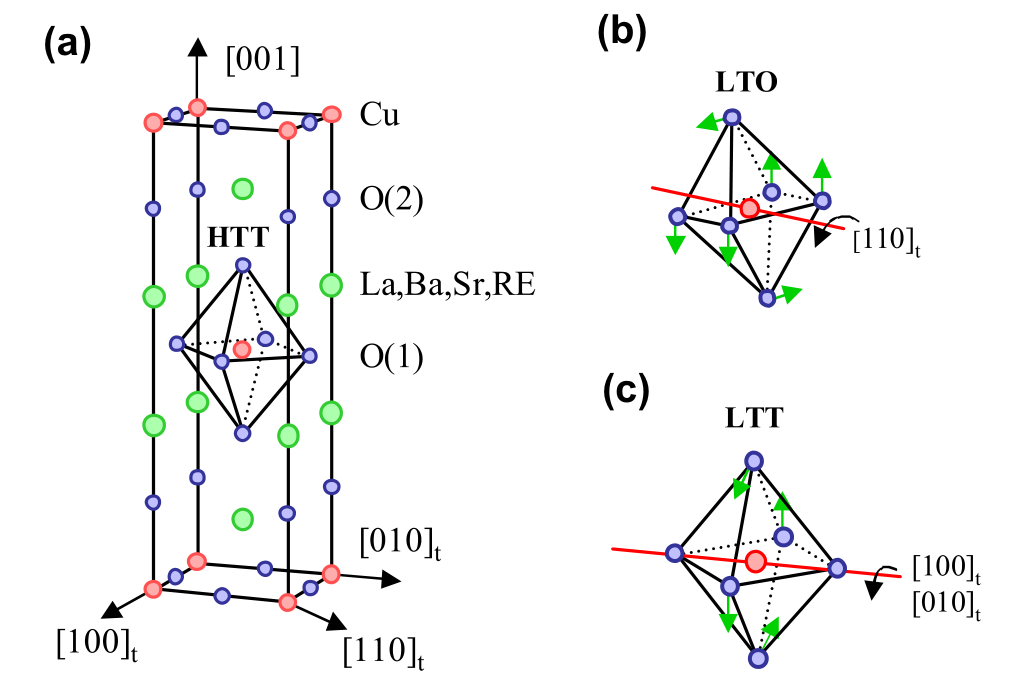
\includegraphics[width=0.8\textwidth]{fig/simulation/crystal_hucker.png}
	\caption[LSCO crystal]{Crystal structure of lanthanum based cuprates based on the HTT conventional cell. From \cite{Hucker2012}. The $Q_1$, $Q_2$ rotations correspond to the LTO tilt in subfigure \textbf{b} and the perpendicular tilt. The LTT tilt in subfigure \textbf{c} corresponds to the case where $Q_1 = Q_2$.\todo[inline]{should update this to orthorhombic coordinate system if time allows...}}
	\label{fig:lscocrystal}
\end{figure}

\section{Coordinate systems}
Having decided on the phases to investigate, we take a short detour to describe the coordinate systems used in real and reciprocal space. Since we are dealing with several electronic and structural phases, we need a common description to compare between phases. In real space, we use the $Q_1$, $Q_2$, $\eta$ description from above and in reciprocal space we use the HTT Brillouin Zone.

\subsection{Octahedral Tilts}
In order to quantify the octahedral tilts for use in simulations, we use the coordinate system sketched in Figure \ref{fig:tilt}. All possible tilts can be described with reference to the lowest symmetry space group (LTLO, Pccn). The octahedra are described with two in-plane oxygens (O$_1$, O$_2$) and one apical oxygen $O_3$ and the Pccn space group is the only one with three inequivalent oxygen atoms. Due to symmetry constrains, a rotation of this octahedron will cause a displacements in the $c$-direction of the in-plane oxygen and in the $a$, $b$ direction of the apical oxygen (a reasonable approximation at small angles). Following \cite{Axe1989}, we define $Q_1$ as a rotation around the (010) axis and $Q_2$ as a rotation around the (100) axis in orthorhombic notation. In more intuitive terms, $Q_1$ `tilts' the octahedron along $a$, while $Q_2$ `tilts' along $b$\todo{show this in the tilt figure}.

\begin{figure}
	\centering
	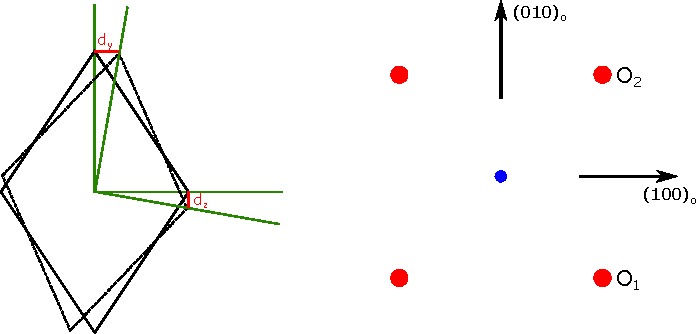
\includegraphics[width=0.8\textwidth]{fig/simulation/tilt.pdf}
	\caption[Geometry of octahedral tilts]{Left: Geometry of octahedral tilts in the with the $c$-axis vertical. Right: Illustration of the two inequivalent in-plane oxygens. The $Q_1$ irreducible representation represents a rotation around the (010) axis while $Q_2$ is a rotation around the (100) axis.\todo[inline]{update this to clearly show x,y,z displacements of O1, O2, O3}}
	\label{fig:tilt}
\end{figure}

By inspection of Figure \ref{fig:tilt}, a $Q_1$ rotation will displace O$_3$ in the $x$-direction and O$_1$, O$_2$ in the negative $z$-direction. A $Q_2$ rotation will displace O$_3$ in the $y$-direction, O$_1$ in the positive $z$-direction and O$_2$ in the negative $z$-direction. If we want to express $Q_1$ and $Q_2$ as angles, the displacements become:

\begin{align*}
\text{O}_3^x &= \text{O}_\text{ap}^z  \sin (Q_1) \frac{c}{a} \\
\text{O}_3^y &= \text{O}_\text{ap}^z \sin (Q_2) \frac{c}{b} \\
\text{O}_1^z &= \frac{1}{4c} \left[ - a \sin (Q_1) + b \sin (Q_2) \right] \\
\text{O}_2^z &= \frac{1}{4c} \left[ - a \sin (Q_1) - b \sin (Q_2) \right] \, ,
\end{align*}

\noindent where $\text{O}^i_j$ is the $i$-component of oxygen $j$ in fractional coordinates. Since these equations uniquely define displacements in terms of tilt angles, we can also find tilt angles from structural displacements from either the apical oxygen:

\begin{align*}
Q_1 &= \sin^{-1} \left( \frac{\text{O}_3^x}{\text{O}_\text{ap}^z} \times \frac{a}{c} \right) \\
Q_2 &= \sin^{-1} \left( \frac{\text{O}_3^y}{\text{O}_\text{ap}^z} \times \frac{b}{c} \right) \, ,
\end{align*}

\noindent or the equatorial oxygen:

\begin{align*}
Q_1 &= \sin^{-1}  \left( - \frac{2c}{a} \times (\text{O}_1^z + \text{O}_2^z) \right) \\
Q_2 &= \sin^{-1}  \left( -\frac{4c}{b} \times \text{O}_2^z - \frac{a}{b} \times \sin (Q_1) \right) \, .
\end{align*}

\noindent To apply an orthorhombic strain $\eta$ to a tetragonal structure with an in-plane lattice parameter $a^\prime$, while keeping the volume constant (which is important when comparing DFT simulations due to Pulay Stress, see section \ref{sec:dft}), the following equations can be used to find the $a$ and $b$ lattice parameters:

\begin{align*}
	a &= \frac{a^\prime}{1+\eta} \\
	b &= (1+\eta) a^\prime \, .
\end{align*}

\noindent These equations can then be used to generate desired tilts and extract tilt angles from any given structure. Since every tilt is defined with respect to only 3 oxygen atoms, these equations require at least Pccn symmetry which is preserved for geometry optimizations and phonon calculations. For lower symmetries (in e.g. MD simulations) we define a `symmetrized average tilt' (see chapter \ref{ch:md}). Code to generate these structures and extract rotation angles from any structure can be found in appendix \ref{app:software}. This methodology can also be used with any software that can generate crystal structures from space group symmetry and fractional coordinates (e.g. ASE \cite{Larsen2017} and VESTA \cite{Momma2008}). The same result can, of course, also be obtained by considering each of the space groups individually and then figuring out how to generate tilts and transform the lattice to a common coordinate system. If one is only interested in atomic coordinates, starting from Pccn is convenient. This way, the atomic indices are also identical.

\subsection{Reciprocal Space: Band Structures}
Band structures are described with respect to the reciprocal lattice. Due to the enlargement of the real-space crystal structure as we move through HTT $\rightarrow$ LTO $\rightarrow$ LTT, the Brillouin Zone (BZ) shrinks by the same amount. Similar to how it is useful to describe our real-space lattice with respect to the Pccn coordinate system, it is useful to describe reciprocal space with respect to a common coordinate system when comparing results. As we can see in Figure \ref{fig:allbz}, the BZ's of HTT, LTO and LTT have vastly different shapes, so it is difficult to superimpose results.

\begin{figure}
	\centering
	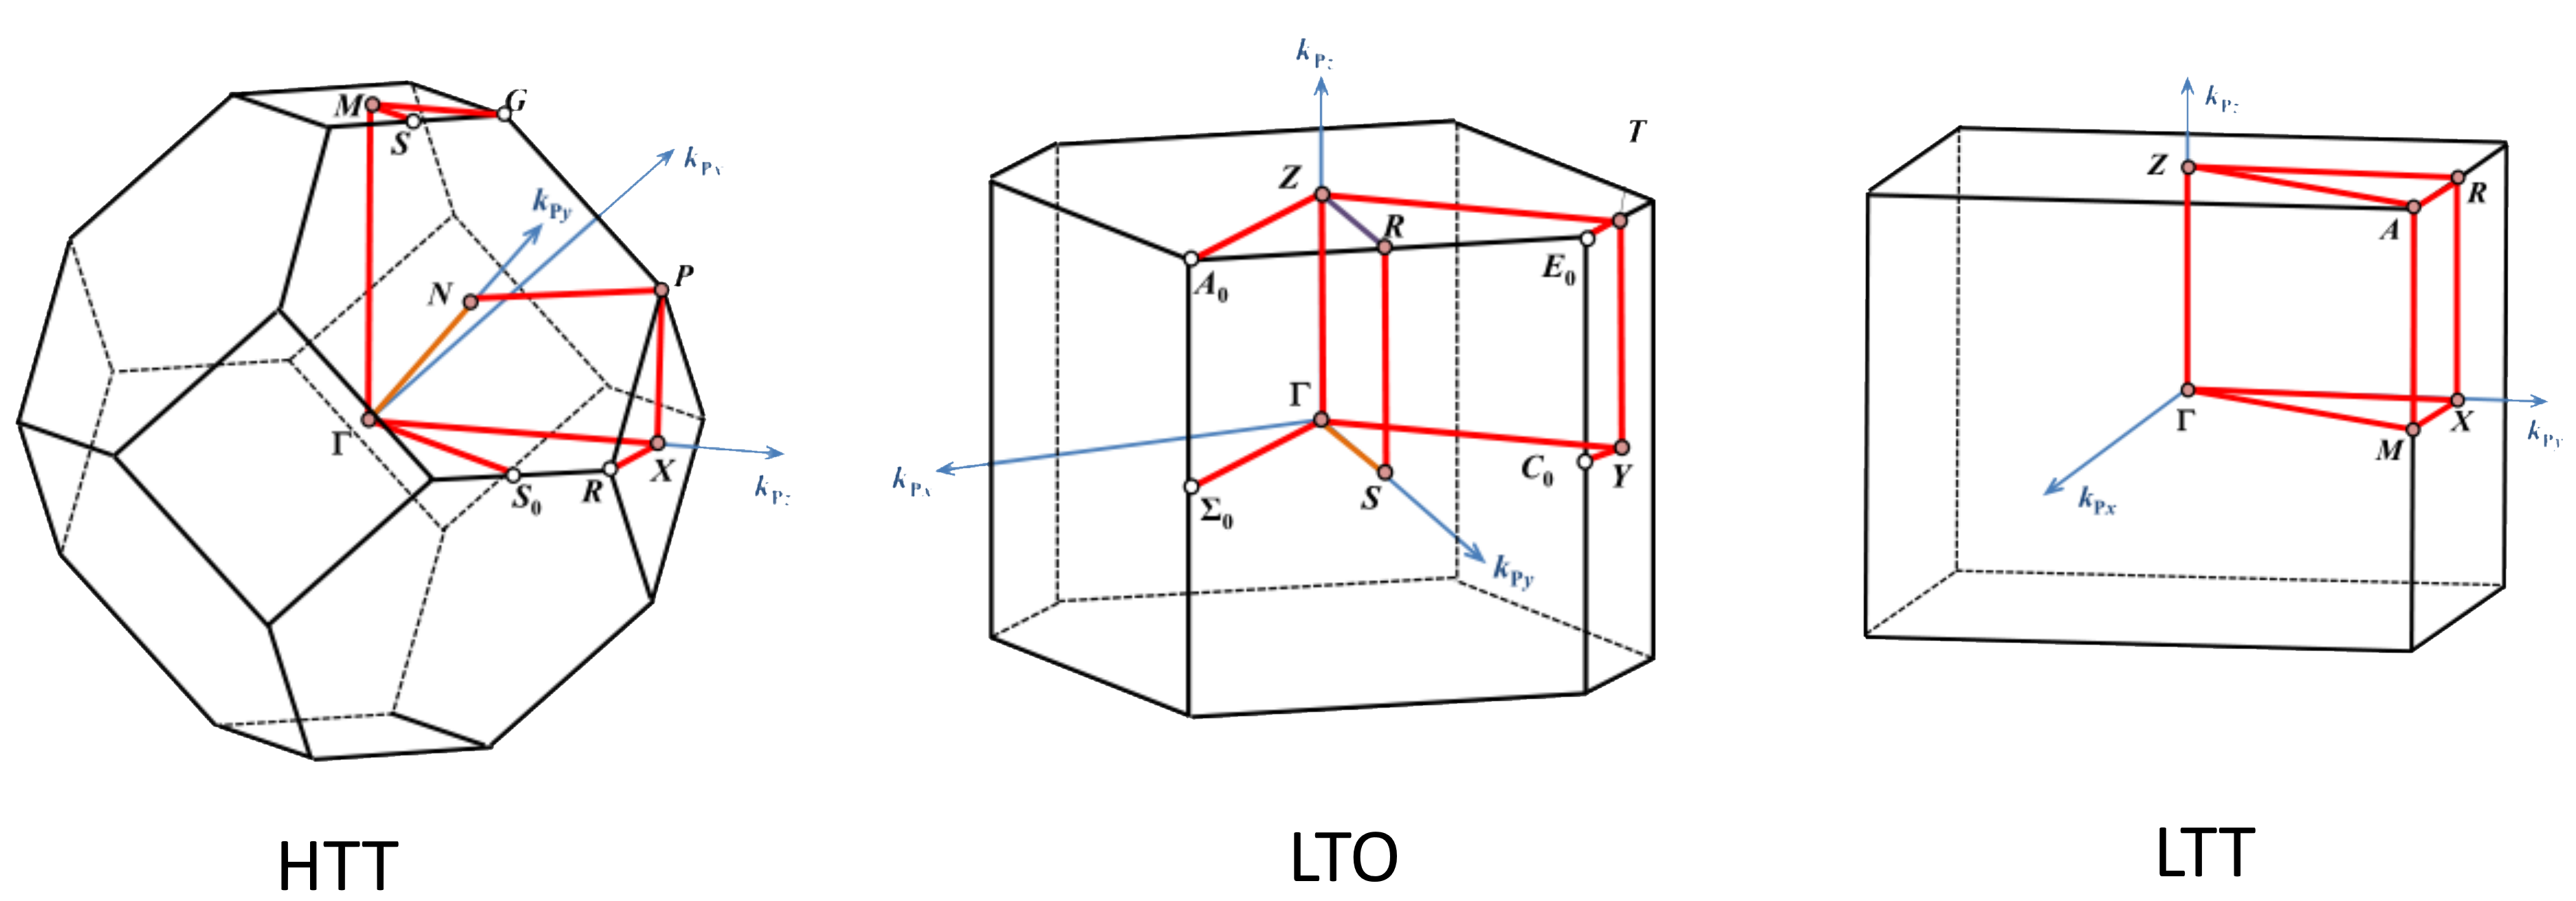
\includegraphics[width=0.8\textwidth]{fig/simulation/BZAll.png}
	\caption[HTT LTO LTT BZs]{Brillouin Zones of the HTT, LTO and LTT phases (see Table \ref{tab:crystalstructures}). Modified from \cite{Hinuma2017}}
	\label{fig:allbz}
\end{figure}

For this reason, we chose a \emph{primitive} tetragonal BZ to describe the HTT phase (note that the shape is different from the actual HTT BZ) and then construct the smaller LTO and LTT BZ's with respect to this construction. The idea is sketched in Figure \ref{fig:band_paths}. This construction also helps emphasize the 2-dimensional nature of the cuprates. In all following simulations, the band labels in Figure \ref{fig:band_paths} will be used, keeping in mind that the nature of high-symmetry points can change depending on the considered structural phase. One example is that the $M$ point, which is the zone boundary of HTT, becomes the zone centre of LTO and would thus usually be denoted $\Gamma$.

\begin{figure}
    \centering
    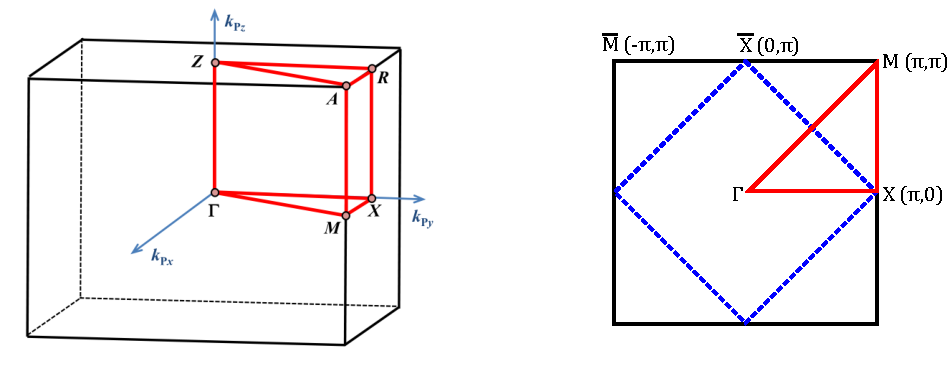
\includegraphics[width=\textwidth]{fig/simulation/band_paths.pdf}
    \caption[Band paths]{\textbf{Left:} BZ of a primitive tetragonal cell with high-symmetry lines. \textbf{Right:} The in-plane BZ with the same labels and the usual $\Gamma$-$X$-$M$-$\Gamma$ path. If the large BZ is the crystallographic HTT phase, then the broken blue lines represent the LTO/LTT/LTLO BZ and we can consider the $\Gamma$-$X$-$\frac{M}{2}$-$\Gamma$ path, since $M$ becomes $\Gamma$ for this (smaller) BZ. In literature the labels are often confused, while $(\pi,\pi)$ and $(\pi,0)$ are universally agreed upon. In any band structure diagrams presented here, the labels in this figure is used.} 
    \label{fig:band_paths}
\end{figure}

While this construction is useful for our intuitive understanding of the different phases, phonon calculations require $k$-vectors with respect to the primitive unit cell. For this reason, we need the transformation matrices from our constructed coordinate system to the primitive HTT and LTO unit cells (the LTT transformation is the identity matrix). This conversion can be done with the following matrices.

\[
\text{PA}_\text{HTT} =  
\begin{pmatrix}
0 & 0 & \frac{1}{2} \\
\frac{1}{2} & \bar{\frac{1}{2}} & 0 \\
\frac{1}{2} & \frac{1}{2} & \bar{\frac{1}{2}}
\end{pmatrix}
\qquad
\text{PA}_\text{LTO} =  
\begin{pmatrix}
\frac{1}{2} & \frac{1}{2} & 0 \\
0 & 0 & 1 \\
\frac{1}{2} & \bar{\frac{1}{2}} & 0
\end{pmatrix}
\]

\noindent these matrices can be used to generate $k$-points starting from the more `intuitive' notation outlined in Figure \ref{fig:band_paths}. For example, the $X$-point ($(\frac{1}{2} \frac{1}{2} 0)$ with respect to our coordinate system) in the HTT phase becomes $(\frac{1}{2} \frac{1}{2} 0) \cdot \text{PA}_\text{HTT} = (\frac{1}{4} \bar{\frac{1}{4}} \frac{1}{4})$.

\section{Strategy}
To find a connection between the structural phases, we start with the highest symmetry phase (HTT) using cell parameters and fractional positions approximated from literature \cite{Radaelli1994a}. The AFM structure is based on La$_2$CuO$_4$ that has been modified in a way such that $\eta=0$ and $Q_1 = Q_2 = 0$. The metallic structure is based on La$_{1.775}$Sr$_{0.225}$CuO$_4$, which is tetragonal (HTT) at \SI{10}{\kelvin}.

The structure is then optimized and we calculate the electronic and phonon band structures. We then break the symmetry by applying a small rigid tilt $Q_2 = \SI{5}{\degree}$ along with small orthorhombic strain $\eta = 0.005$, resulting in the LTO phase which we then optimize and finally perform the same set of calculations. A HTT-LTT transformation is performed in a similar fashion with $Q_1 = Q_2 = \SI{5}{\degree}$ and $\eta = 0$. This procedure is then performed in parallel for the anti-ferromagnetic solution using LDA+U and the metallic solution. The resulting band structures, density-of-states and total energies are then analysed and validated against experimental data. 

All calculations in this chapter is performed on La$_2$CuO$_4$ in the conventional orthorhombic unit cell, which corresponds to the primitive Pccn lattice that we use to generate the structures. This cell contains four formula units and is large enough to accommodate anti-ferromagnetism. Since VASP can handle symmetry through the \texttt{ISYM} keyword, we don't need an input cell corresponding to the primitive cell of the considered structural phase. Before starting any `production' DFT calculation, it is advantageous to benchmark certain computational parameters in order to get an idea of how well-behaved the SCF convergence is and what energy scales we can expect to probe.

\section{Benchmarking}\label{sec:sim_benchmark}
When performing DFT calculations in VASP there are a few parameters that have significant impact on the precision of the calculation. Increasing the precision also results in significantly longer computation time, so it is important to find a compromise. 

Figure \ref{fig:sim_bench_afm} shows a benchmark of AFM LCO with respect to the $k$-point mesh and smearing width $\sigma$. Since there are no states at the Fermi level, the smearing width converges rather quickly, and we can safely use a value of $\sigma = \SI{0.1}{\eV}$. The $k$-point density also converges rather quickly, and we achieve a precision of \SI{0.1}{\milli\eV} using a fairly coarse MP-grid of $8\times 8 \times 4$ (7168 $k$-points per reciprocal atom). In AFM LCO we also checked the effect on electronic structure due to the on-site repulsion $U$. The result is shown in Table \ref{tab:ldau} and the values of $U=\SI{8}{\eV}$, $J=\SI{0.8}{\eV}$ are chosen based on the proximity to experimental evidence \cite{Vaknin1987, Uchida1991} and previous theoretical studies of the La$_2$CuO$_4$ system, where the values of $U$ and $J$ where found self-consistently \cite{Anisimov2004,Anisimov1991}.

\begin{figure}
    \centering
    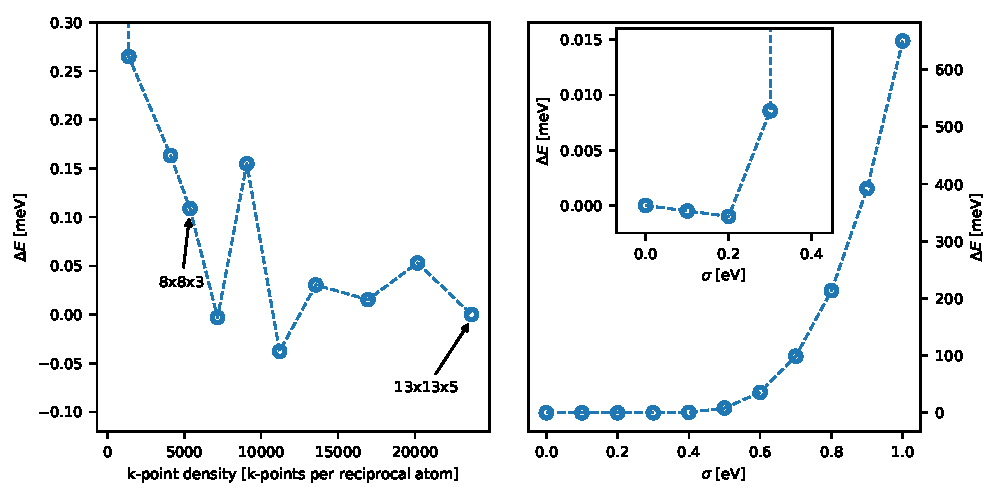
\includegraphics[width=\textwidth]{fig/simulation/convergence_afm.pdf}
    \caption[Simulation Benchmarks: GGA+U]{Simulation Benchmarks: GGA+U with $U=\SI{8}{\eV}$ and $J=\SI{0.8}{\eV}$. \textbf{Left:} Energy as a function of k-point density with $\sigma=\SI{0.1}{\eV}$. $\Delta E$ is total energy (with entropy) with respect to the $13 \times 13 \times 5$ mesh. \textbf{Right:} $\Delta E = E_0 - E$ as a function of Gaussian smearing $\sigma$, $E$ is the total energy and $E_0$ is the energy where $\sigma=0$ calculated with the tetrahedron method (\texttt{ISMEAR=-5} in VASP).}
    \label{fig:sim_bench_afm}
\end{figure}

\begin{table}[b]
	\centering
	\caption[LDA+U Benchmarking]{LDA+U Benchmarking of the parameters $U$ and $J$ calculated with \texttt{LDAUTYPE=4} in the HTT phase of La$_2$CuO$_4$. Experimentally the Cu moment is $(0.48 \pm 0.15) \, \mu_\text{B}$ \cite{Vaknin1987} and the optical gap is $\approx \SI{2}{\eV}$ \cite{Uchida1991}. As a reasonable compromise we chose $U=\SI{8}{\eV}$ and $J=\SI{0.8}{\eV}$, a set of values also used in a previous study of the same system \cite{Anisimov2004}.}
	\label{tab:ldau}
	\begin{tabular}{@{}llll@{}}
		\toprule
		U [eV] & J [eV] & Moment [$\mu_\text{B}$] & Optical gap [eV] \\ \midrule
		4.0    & 0.4    & 0.330       & 0.348    \\
		6.0    & 0.6    & 0.481       & 1.016    \\
		8.0    & 0.8    & 0.588       & 1.686    \\
		10.0   & 1.0    & 0.676       & 1.877    \\
		12.0   & 1.2    & 0.755       & 2.042    \\ \bottomrule
	\end{tabular}
\end{table}

Due to partial occupancies, metallic systems are generally more sensitive to $k$-point density and smearing width/method. For this reason, we performed a more comprehensive set of benchmarks as shown in Figure \ref{fig:sim_bench_para}. While the numerical fluctuations are within a few meV, the precision on total energy is decreased by a few orders of magnitude. Based on these results, we evaluate the metallic simulations at twice the $k$-point density with a mesh of $16 \times 16 \times 8$ (57344 $k$-points per reciprocal atom).

\begin{figure}
    \centering
    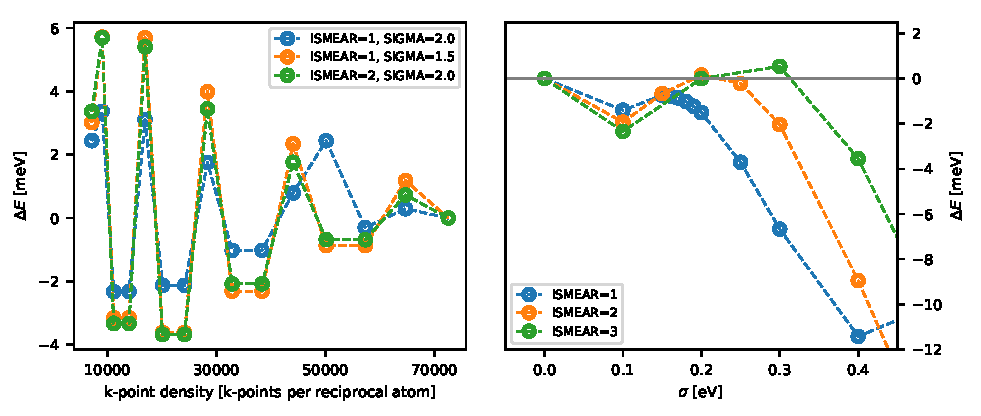
\includegraphics[width=\textwidth]{fig/simulation/convergence_metal.pdf}
    \caption[Simulation Benchmarks: Paramagnet/Metal]{Simulation Benchmarks: Paramagnet/Metal. Note the significant variation in energy compared to the insulating case, even with much higher k-point density. \textbf{Left:} Energy as a function of k-point density for three combinations values of $\sigma$ and smearing type. $\Delta E$ is total energy (with entropy) with respect to the $18 \times 18 \times 8$ mesh. \textbf{Right:} $\Delta E$ as a function of $\sigma$ with the Methfessel-Paxton method (orders 1, 2, 3) while using a $16 \times 16 \times 8$ k-point mesh (57344 k-points per reciprocal atom). $\sigma=0$ corresponds to the tetrahedron method (\texttt{ISMEAR=-5}). Below $\sigma = \SI{0.4}{\eV}$ the entropy term is \SI{0.5}{\milli\eV} per atom or lower, so forces should be well-behaved.}
    \label{fig:sim_bench_para}
\end{figure}

%\begin{table}[b]
%	\centering
%	\begin{tabular}{@{}lllll@{}}
%		\toprule
%		& HTT & HTT (metal)  & LTO    & LTT    \\ \midrule
%		a [\AA]         & 5.32 & 5.31 & 5.34   & 5.37   \\
%		c [\AA]         & 12.99 & 13.05 & 13.01  & 12.93  \\
%		O3(z)      & 0.184 & 0.185 & 0.185  & 0.184  \\
%		La(x)      & 0     & 0 & 0      & -0.009 \\
%		La(y)      & 0     & 0 & -0.012 & -0.009 \\
%		La(z)      & 0.362 & 0.362 & 0.361  & 0.361  \\
%		$\eta$ ($\times 100$) & 0  & 0 &  1.465  & 0      \\
%		Q1 (degrees)        & 0 & 0 &  0      & 4.6125 \\
%		Q2 (degrees)        & 0 & 0 &  5.786  & 4.6125 \\ 
%		degrees of freedom & 2 & 2 & 5 & 5 \\ \bottomrule
%	\end{tabular}
%	\caption[HTT, LTO, LTT: Structural parameters]{HTT, LTO, LTT: Structural parameters, defined with a minimal set of parameters based on results from simulations. Q1/Q2 are taken as the average angle from equatorial and apical tilt. The fractional positions of O1, O2 and O3 are completely described using Q1, Q2 and O3(z), Cu is allways at (0,0,0) and $\eta = \frac{b-a}{b+a}$ uniquely defines any difference between $a$ and $b$. In the generation of structures, the Pccn (LTLO) space group is used. Degrees of freedom refers to the atomic positions only. The description of our system in terms of Q1/Q2 thus removes one degree of freedom by coupling the apical and equatorial oxygen.}
%	\label{tab:struct_par}
%\end{table}

\subsection{Electronic Structure}
While we are generally interested in lattice dynamics, a DFT calculation is leveraging the electronic structure in any simulation. It is thus worthwhile to check if the electronic structure, at least approximately, represents reality in the benchmarking phase of our simulations. In the cuprates, it is well known that DFT is unable to explain the peculiarities in the superconducting phase. However, we can get fairly close in the limit of zero doping (AFM Mott Insulator) and over-doping (fermi liquid). Figure \ref{fig:edos_htt} compares the electronic density of states of the Mott Insulator and fermi liquid for our chosen functionals. We clearly see how the DFT+U opens a gap by pushing states below the Fermi level. We also notice that, in terms of DOS, the functionals behave qualitatively similar.  

\begin{figure}
    \centering
    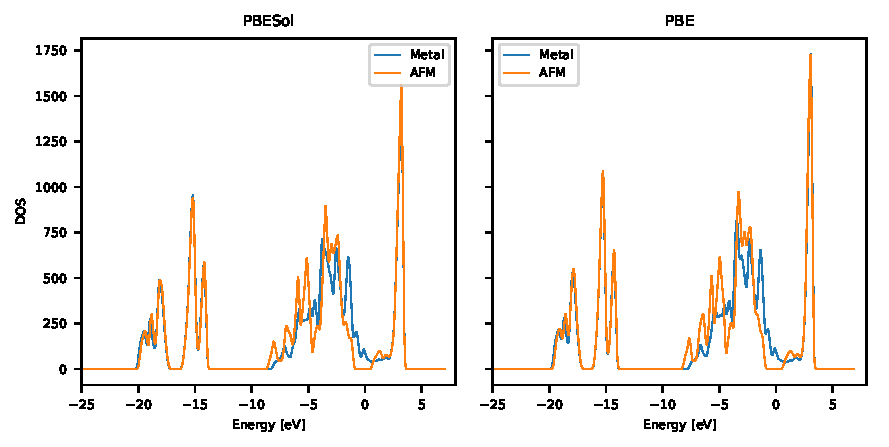
\includegraphics[width=\textwidth]{fig/simulation/htt_dos.pdf}
    \caption[Electronic DOS: Metal and AFM]{Electronic density of states for HTT phase with two different functionals in a metallic (paramagnetic) and AFM (GGA+U) states. The two functionals appear to describe the system identically. The AFM state is shifted by \SI{-1}{\eV} for comparative purposes (which is why the Fermi level is in the middle of the gap).}
    \label{fig:edos_htt}
\end{figure}

To further illustrate this point, Figure \ref{fig:bs_afm1} and \ref{fig:bs_metal} shows the electronic band structures coloured by atomic projections in the AFM and metallic state, respectively. We now notice that DFT+U is pushing the Cu states down by about \SI{8}{\eV}, as expected from the on-site repulsion $U$. Comparing our band structures to literature we have, as expected, a qualitative agreement in both the AFM \cite{Lane2018} and metallic \cite{Matt2018, Horio2018} cases. As mentioned in section [XX], the metallic band structures also agree quite well with experimental ARPES studies. The question of LDA+U being an appropriate model for the undoped AFM system is still not settled \cite{Damascelli2003}.\todo{find a more recent paper.}

% \begin{figure}
%     \centering
%     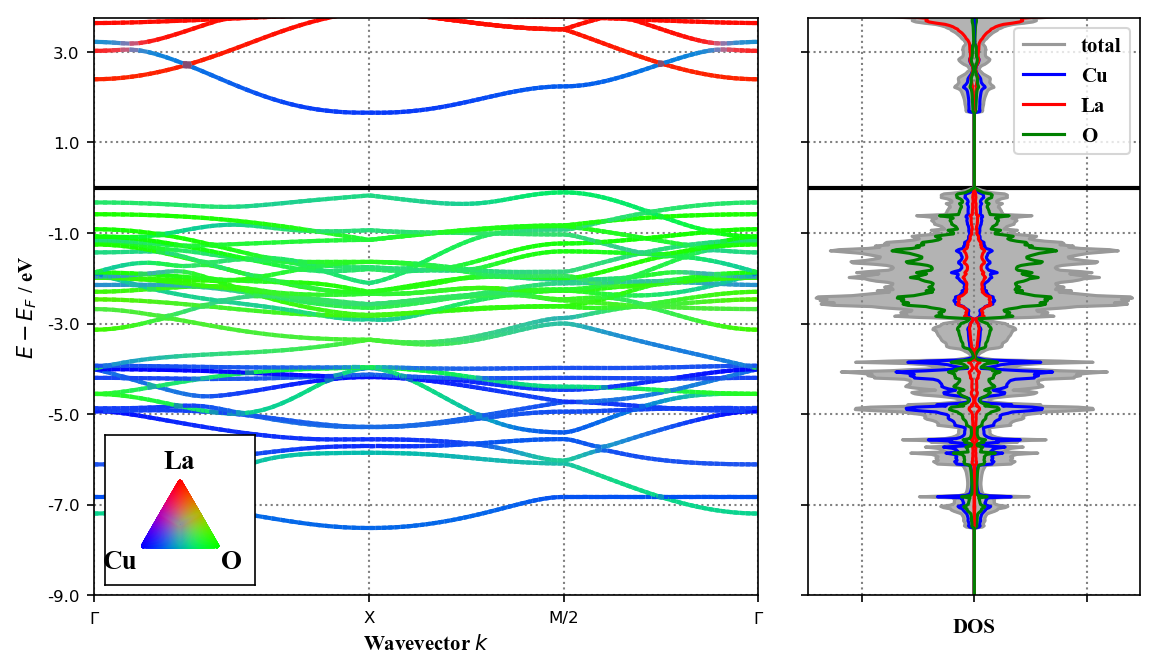
\includegraphics[width=\textwidth]{fig/simulation/bs_afm2.png}
%     \caption[GGA+U: AFM Electronic Band Structure]{GGA+U: AFM Electronic Band Structure of the Bmab LTO structure along the $\Gamma$-$X$-$\frac{M}{2}$-$\Gamma$ path (LTO high symmetry lines). The upper and lower Hubbard bands are clearly visible and are separated by \SI{8}{\eV} as expected.}
%     \label{fig:bs_afm2}
% \end{figure}

\begin{figure}
   \centering
   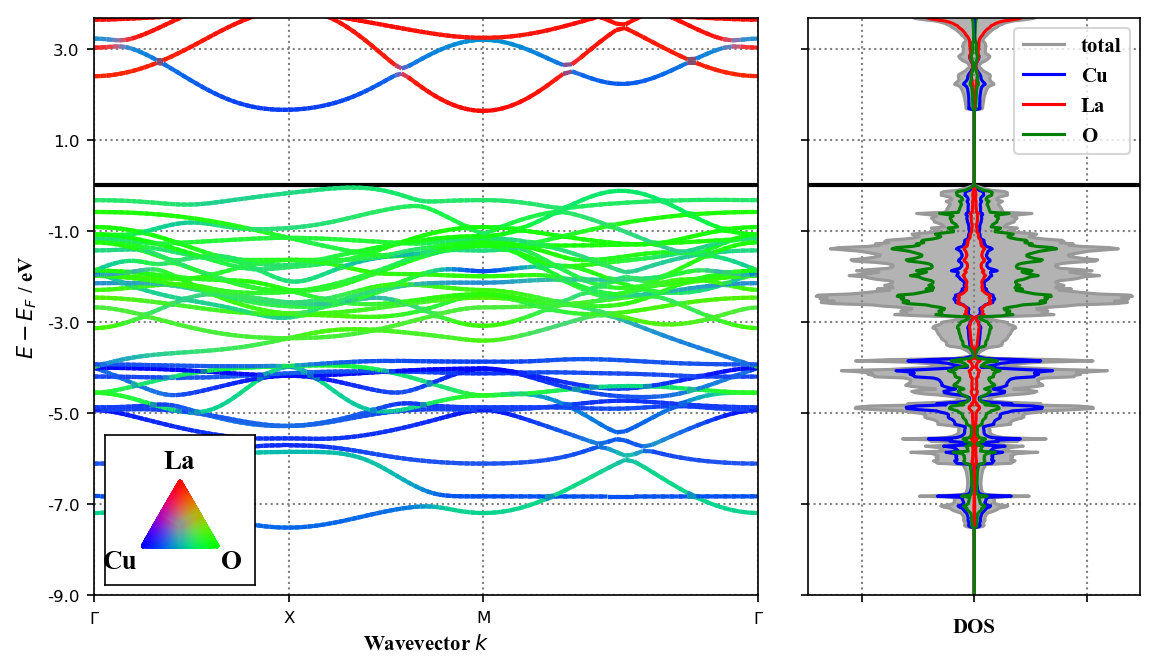
\includegraphics[width=\textwidth]{fig/simulation/bs_afm1.png}
   \caption[GGA+U: AFM Electronic Band Structure]{GGA+U: AFM Electronic Band Structure of the Bmab LTO structure along the $\Gamma$-$X$-$M$-$\Gamma$ path (HTT high symmetry lines). The upper and lower Hubbard bands are clearly visible and are separated by \SI{8}{\eV} as expected.}
   \label{fig:bs_afm1}
\end{figure}

\begin{figure}
    \centering
    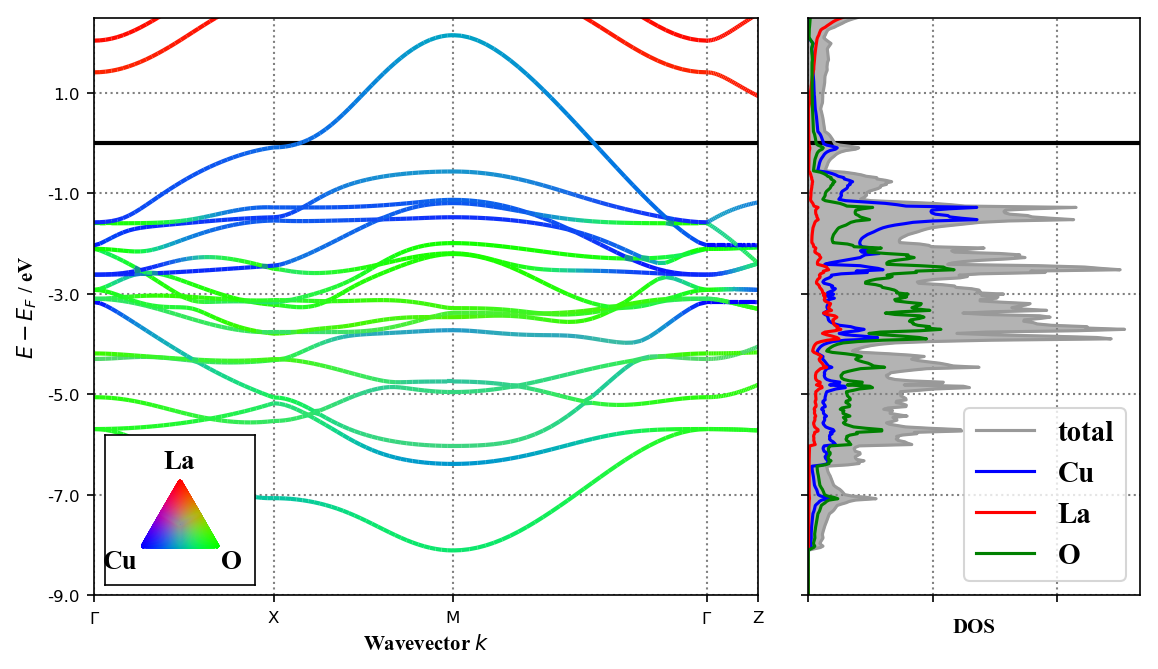
\includegraphics[width=\textwidth]{fig/simulation/bs_metal.png}
    \caption[GGA: Metallic Electronic Band Structure]{Metallic Electronic Band Structure of the I4/mmm HTT structure. Path is through the high-symmetry points as defined in Figure \ref{fig:band_paths} with respect to the conventional unit cell. The $\Gamma$-$Z$ path is shown to illustrate the 2-dimensional nature of the electronic structure (The dispersion is relatively flat).}
    \label{fig:bs_metal}
\end{figure}

\section{Geometry optimization}\label{sec:sim_geomopt}
Having settled on a set of appropriate computational parameters, we can proceed with the original goal of optimizing the geometry of the various structural phases. Optimizing geometry in VASP can be performed with 3 different algorithms controlled by the \texttt{IBRION} tag:

\begin{enumerate}
	\item RM-DIIS
	\item Conjugate Gradient (CG)
	\item Damped molecular dynamics
\end{enumerate}

\noindent All algorithms requires to set the \texttt{POTIM} tag which controls the step-size. Usually the default value of 0.5 is reasonable. Damped molecular dynamics requires a damping factor in addition, set by the \texttt{SMASS} tag. For this reason RM-DIIS and CG require less user intervention and are good first choices. While RM-DIIS is usually a good choice for systems close to equilibrium, it struggles with rigid unit modes such as octahedral tilts in perovskites. Since these tilts are at the centre of our investigation, we use CG in most cases.

The optimization routine is constrained by the point group symmetry as determined by VASP. The \texttt{ISIF} tag controls how the positions, cell shape and cell volume is updated during the optimization. It might seem obvious to simply optimize everything, but for complex problems convergence can be problematic. In addition, changing the cell volume affects the plane-wave basis set. Intuitively, this can be understood through thinking of the plane waves as standing waves in our finite box. Changing the size of the box necessarily changes the plane waves. This is also true when considering changes to the cell shape, but in a less significant way. These effects are known as `Pulay stress' \cite{zotero-1453} and are important to keep in mind when performing geometry optimizations. The effect of this can be avoided by changing the size of the basis set through the energy cut-off or by avoiding volume relaxations all together. In practice, there are two primary strategies for getting accurate geometry optimizations in VASP. The first is a step-wise optimization of parameters in the scheme

\begin{quote}
	Coordinates $\rightarrow$ Coordinates/Shape $\rightarrow$ Coordinates/Shape/Volume, 
\end{quote}

\noindent where we are susceptible to severe Pulay stress only in the last step. The second is perform successive coordinate+shape optimizations at a set of fixed volumes and fit the resulting volume-energy curve to an equation-of-state (EOS). This avoids the most significant contribution to Pulay stress by never performing a volume optimization explicitly. While this method is more computationally expensive, it is more accurate and provides us with additional information about volume-dependent behaviour such as the bulk modulus, tilt patterns and orthorhombic strain. In practice we use the exponential EOS formulated by \citeauthor{Vinet1987} \cite{Vinet1987}:

\begin{align*}
E(V) &= E_0 + \frac{2B_0V_0}{\left(B_0^\prime-1\right)^2} \\
&\times \left\lbrace 2 -\left[ 5 + 3\left( \frac{V}{V_0}\right)^\frac{1}{3} (B_0^\prime -1)  -3B_0^\prime \right] \right. \left. \exp \left[ -\frac{3}{2} \left( B_0^\prime-1\right)\left[\left( \frac{V}{V_0}\right)^\frac{1}{3} -1\right]\right]\right\rbrace
\end{align*}

\noindent where $V_0$ is the equilibrium volume, $B_0$ is the bulk modulus and 

\begin{equation*}
B_0^\prime = \left( \frac{\partial B_0}{\partial P}\right)_T \, .
\end{equation*}

\noindent There exists several alternative energy-volume EOS formulations in literature \cite{Murnaghan1944, Birch1947, Poirier1998} designed for different conditions and materials. By testing several of these formulations on the same data, we get practically indistinguishable results, so the choice of the Vinet formula is somewhat arbitrary. In practice, roughly 10 volumes ranging from $\pm 5\%$ of the equilibrium are chosen, adding more volumes to fill out the graph if necessary. While performing the fits, we extract information about the volume-dependent tilt angles and cell ratios.

Since forces are more susceptible to the energy cut-off, test were performed at the recommended cut-off, 1.3 times the cut-off and 2 times the cut-off. While the latter seems extreme at first glance, our phonon calculations show that we iron out certain artefacts of low-energy modes by using a large cut-off. A similar effect was seen in simulations of CsSnI$_3$ \cite{DaSilva2015}, a perovskite with distorted octahedra. As we shall see, the forces related to tilting octahedra is quite subtle in DFT.

\subsection{Geometry of AFM LCO}
We performed equation-of-state fits to AFM La$_2$CuO$_4$ in all three structural phases. Figure \ref{fig:eos_afm_all} shows the Energy-Volume fits, Figure \ref{fig:eos_ratios_afm} shows the volume dependence of the cell ratios and Figure \ref{fig:angles_afm} shows how the angles in the LTO and LTT phases change as a function of volume. Contrary to experiment, the LTO phase is energetically unfavourable and the favoured phase is LTT. In the tetragonal phases, the optimal $c/a$ ratio is reduced as a function of volume while the LTO phase has a maximum at optimal volume. The orthorhombicity in the LTO phase increases as a function of volume and tilts in the LTO and LTT phases increase wit increasing volume. Figure \ref{fig:angles_afm} additionally reveals that the $Q_1$ and $Q_2$ are not completely rigid, consistent with experiment \cite{Radaelli1994a}. Intuitively, it is `easier' to move the apical oxygen due to the rocksalt-layer being less dense. The observations on LTO are consistent with structural studies of LSCO under pressure \cite{Takahashi1994}, where both the orthorhombic strain and tilt angle are decreased with increasing pressure.

\begin{figure}
    \centering
    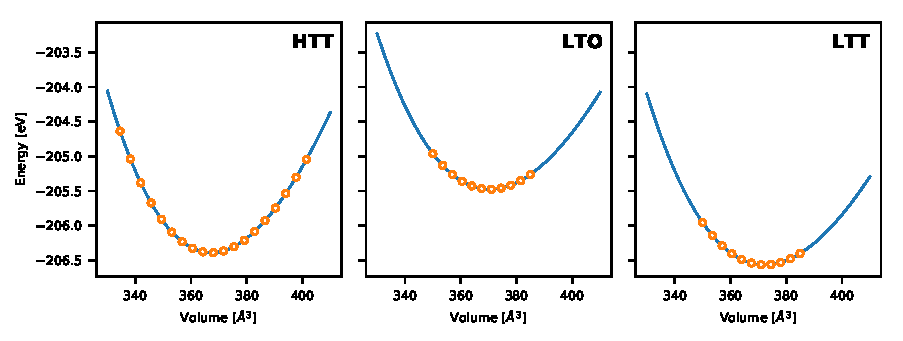
\includegraphics[width=\textwidth]{fig/simulation/eos_all.pdf}
    \caption[AFM: Equation-of-state fits]{Equation-of-state fits (AFM). Optimal volume of simulated structures are found by performing optimization of fractional coordinates and cell shape at a series of fixed volumes. The resulting Energy/Volume curve is then fit to a Vinet exponential equation of state \cite{Vinet1987}. This is done for the HTT, LTO and LTT phases with the PBESol functional.}
    \label{fig:eos_afm_all}
\end{figure}

\begin{figure}
    \centering
    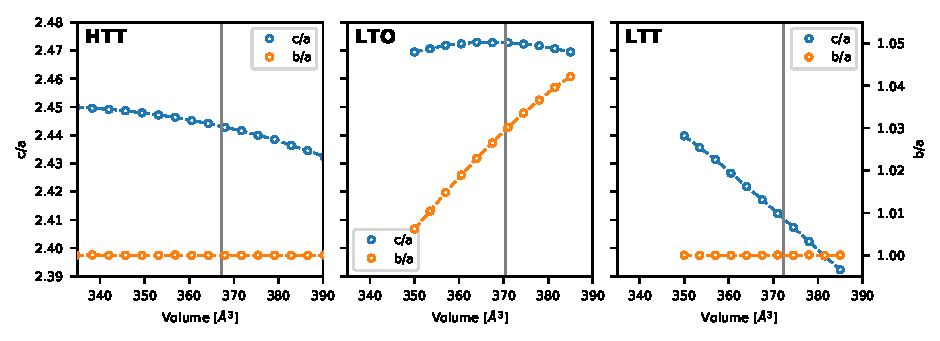
\includegraphics[width=\textwidth]{fig/simulation/ratio_all.pdf}
    \caption[AFM: Cell ratios during EOS fits]{Cell Ratios (AFM). During the equation-of-states fits from Figure \ref{fig:eos_afm_all}, the cell shape is modified, changing the $b/a$ ratio (orthorhombicity) and $c/a$ ratio (larger values correspond to a cell that is elongated along $c$). Due to symmetry $b/a = 1$ for the HTT and LTT phases. Vertical line is the optimal volume from the fit.}
    \label{fig:eos_ratios_afm}
\end{figure}

\begin{figure}
    \centering
    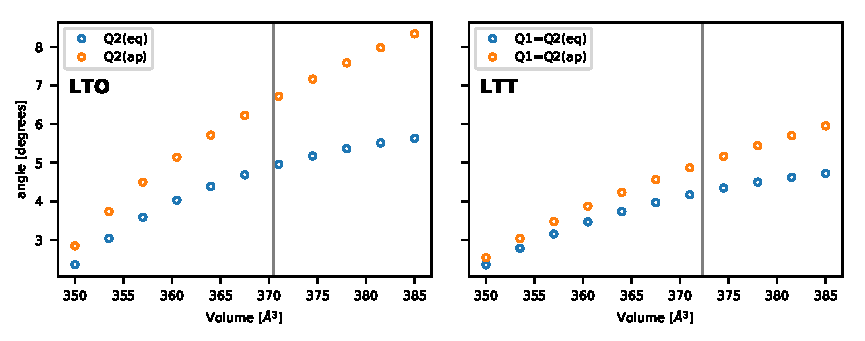
\includegraphics[width=\textwidth]{fig/simulation/angles_lto_ltt.pdf}
    \caption[AFM: LTO/LTT angles during EOS fits]{LTO/LTT Angles (AFM) During equation-of-state fits, we record the tilt angles for the LTO and LTT phase. Here, they are plotted as a function of Volume. Note that for LTO $Q_1=0$ and for LTT $Q_1=Q_2$. However, the rotation angle is measured differently from the equatorial (eq) and apical (ap) oxygen. The difference in values can be thought of as `non-rigidity' of the rotation.}
    \label{fig:angles_afm}
\end{figure}

\subsection{Geometry of metallic LCO}
The same geometry optimization was performed in the metallic state of La$_2$CuO$_4$. EOS fits are shown in Figure \ref{fig:eos_metal_all}, cell ratios are shown in Figure \ref{fig:eos_ratios_metal} and the LTO/LTT angles are shown in Figure \ref{fig:angles_metal}. Qualitatively, we notice very similar behaviour to AFM LCO with regards to cell ratios and tilt angles, but for these calculations LTT and LTO are the preferred phases with very similar total energies. This is inconsistent with, the electronically well-described, over-doped phase where the structure is actually HTT at low temperatures \cite{Radaelli1994a}. Since the difference is roughly $\SI{0.2}{\eV} = \SI{200}{\milli\eV}$ and our uncertainty in energy is around \SI{2}{\milli\eV} (see Figure \ref{fig:sim_bench_para}), it is hard to imagine a scenario where the discrepancy is due to numerical noise, especially since the calculations were performed with a very dense $k$-point mesh of $16 \times 16 \times 8$. It is, however, worth noting that the evaluation of forces is quite different between metallic and insulating solutions in plane wave DFT.

\begin{figure}
    \centering
    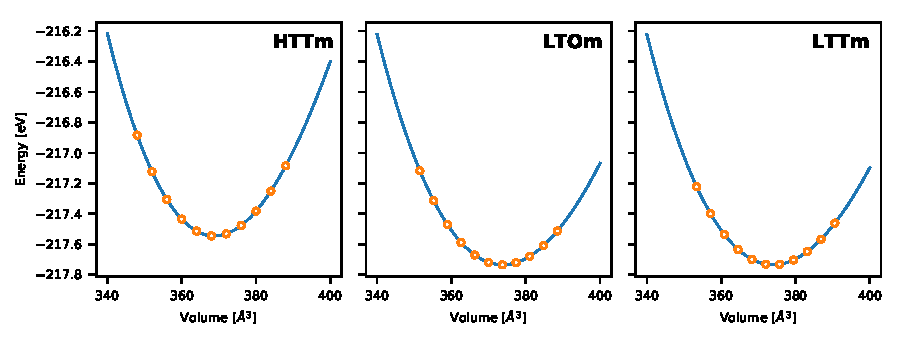
\includegraphics[width=\textwidth]{fig/simulation/eos_metal_all.pdf}
    \caption[Metal: Equation-of-state fits]{Equation-of-state fits (Metal). Optimal volume of simulated metallic structures are found by performing optimization of fractional coordinates and cell shape at a series of fixed volumes. The resulting Energy/Volume curve is then fit to a Vinet exponential equation of state \cite{Vinet1987}. This is done for the HTT, LTO and LTT phases with the PBESol functional.}
    \label{fig:eos_metal_all}
\end{figure}

\begin{figure}
    \centering
    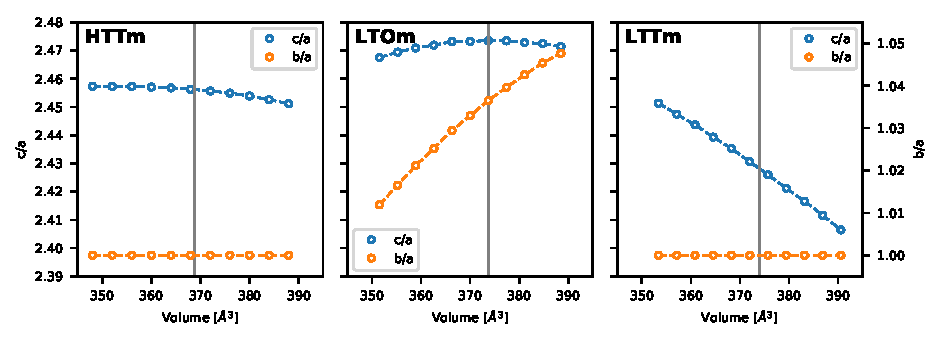
\includegraphics[width=\textwidth]{fig/simulation/ratio_metal_all.pdf}
    \caption[Metal: Cell ratios during EOS fits]{Cell ratios (Metal). During the equation-of-states fits from Figure \ref{fig:eos_metal_all}, the cell shape is modified, changing the $b/a$ ratio (orthorhombicity) and $c/a$ ratio (larger values correspond to a cell that is elongated along $c$). Due to symmetry $b/a = 1$ for the HTT and LTT phases. Vertical line is the optimal volume from the fit.}
    \label{fig:eos_ratios_metal}
\end{figure}

\begin{figure}
	\centering
	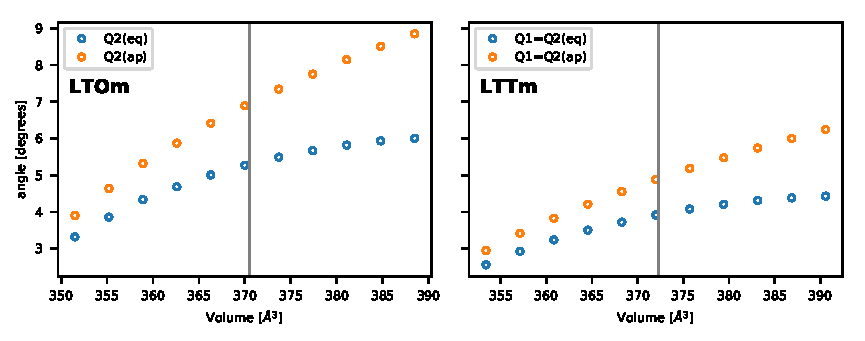
\includegraphics[width=\textwidth]{fig/simulation/angles_metal_lto_ltt.pdf}
	\caption[Metal: LTO/LTT angles during EOS fits]{LTO/LTT angles (Metal). During equation-of-state fits, we record the tilt angles for the LTO and LTT phase. Here, they are plotted as a function of Volume. Note that for LTO $Q_1=0$ and for LTT $Q_1=Q_2$. However, the rotation angle is measured differently from the equatorial (eq) and apical (ap) oxygen. The difference in values can be thought of as `non-rigidity' of the rotation.}
	\label{fig:angles_metal}
\end{figure}


\subsection{Summary of geometry optimization}
A summary of all the geometry optimizations are shown in Table \ref{tab:sim_struct}. Additional data from simulations with a different functional have been added to this table. We notice that the PBE functional finds a volume closer to experimental value, but phonon calculations show a more consistent behaviour of the PBESol functional.

\begin{table}
	\centering
	\caption[Simulation Structure Results]{Resulting structure due to EOS fits to various structural phases and functionals. The two values given for $Q_1$/$Q_2$ are angles calculated from equatorial and apical oxygens, respectively. Interestingly, in terms of energy LTT $<$ HTT $<$ LTO, while the phonons are `more unstable' for HTT than LTO (See Figures \ref{fig:htt_bands}, \ref{fig:lto_bands}, \ref{fig:ltt_bands}). For the metallic cases, we note the optimal geometry is similar to the magnetic case. While the energy is lower, it is not meaningful to compare total energies between GGA+U and GGA.}
    \label{tab:sim_struct}
    \begin{tabular}{lllllllllll}
\toprule
structure &  phase & encut &      XC &       E0 &       V0 &    c/a &    $\eta$ &     $Q_1$ &     $Q_2$ \\
\midrule
      HTT &    afm &   520 &     PBE & -194.352 &  383.410 &  2.431 &  0.000 &  0.000 &  0.000 \\
      HTT &    afm &   800 &     PBE & -194.494 &  383.297 &  2.430 &  0.000 &  0.000 &  0.000 \\
      HTT &    afm &   800 &  PBESol & -206.390 &  367.310 &  2.443 &  0.000 &  0.000 &  0.000 \\
      LTO &    afm &   800 &  PBESol & -205.476 &  370.500 &  2.437 &  1.465 &  0.000 &  5.786 \\
      LTT &    afm &   800 &  PBESol & -206.565 &  372.282 &  2.410 &  0.000 &  4.612 &  4.612 \\
      HTT &  metal &   800 &  PBESol & -217.546 &  368.774 &  2.456 &  0.000 &  0.000 &  0.000 \\
      LTO &  metal &   800 &  PBESol & -217.735 &  373.793 &  2.430 &  1.795 &  0.000 &  6.421 \\
      LTT &  metal &   800 &  PBESol & -217.735 &  373.948 &  2.428 &  0.000 &  4.528 &  4.528 \\
\bottomrule
\end{tabular}

\end{table}

\section{Phonons}
Phonons are calculated using the Phonopy software using the finite displacement (also known as the direct method or the frozen phonon method). Details on the methodology is given in section \ref{sec:phononpractical}. Phonon calculations were performed on both metallic and AFM LCO in the HTT, LTO and LTT structural phases. We use the same computational parameters as in the preceding sections, but expand to a $2 \times 2 \times 1$ supercell in order to compute phonon energies at finite values of $\bm{q}$. Since the cell is expanded, we reduce the $k$-point mesh to $4 \times 4 \times 4$ for both the metallic and magnetic solutions. While it would be preferable to perform the metallic simulation at a higher $k$-point density, memory requirements became a problem when performing computations on a supercell with P1 symmetry. While we can rely on most of the computational parameters chosen/obtained in the preceding sections, we check the effect of functional choice and energy cut-off (\texttt{ENCUT}) on phonon bands since these are more susceptible to instabilities in forces. In Figure \ref{fig:pbe_bands}, we show the phonon band structure in the AFM phase with \texttt{ENCUT=520} and \texttt{ENCUT=800}. While the effect of increasing the plane wave cut-off is small, we see immediately that it fixes some unstable modes at $\Gamma$. While we do expect instabilities at the $M$ point in the HTT phase, the results could be improved.

\begin{figure}
	\centering
	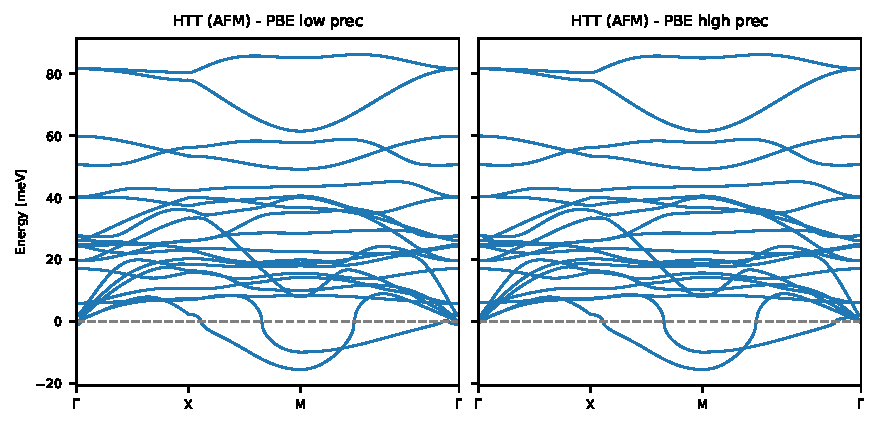
\includegraphics[width=\textwidth]{fig/simulation/htt_pbe_bands.pdf}
	\caption[PBE Bands: Comparison wrt ENCUT]{Phonon band structure of LCO in the HTT phase using the PBE functional with a \SI{520}{\eV} (low prec) and \SI{800}{\eV} (high prec) plane wave cut-off. Both simulations are performed using a magnetic electronic structure within the DFT+U formalism.}  
	\label{fig:pbe_bands}
\end{figure}

For this reason, we keep the \SI{800}{\eV} cut-off and perform the same phonon calculation using the PBESol \cite{Csonka2009} functional. This functional has been successful for phonon calculations in other perovskite systems with tilt disorder \cite{DaSilva2015}, so it is a likely candidate for improvement. 

\subsection{Band structures}
Figure \ref{fig:htt_bands} shows phonon band structures in the HTT phase using both AFM and metallic electronic structures. We immediately notice improvements on two fronts. First, the low-energy modes are `more stable' and the low-energy optic modes have been moved up. In addition the unstable modes are localized around $M$ where we expect a structural phase transition. Second, the high-energy bond-stretching mode ($\Gamma$-$X$) has increased in energy and is much closer to experimental values. In addition, we reproduce the softening of this mode at $X$ due to doping.

\begin{figure}
	\centering
	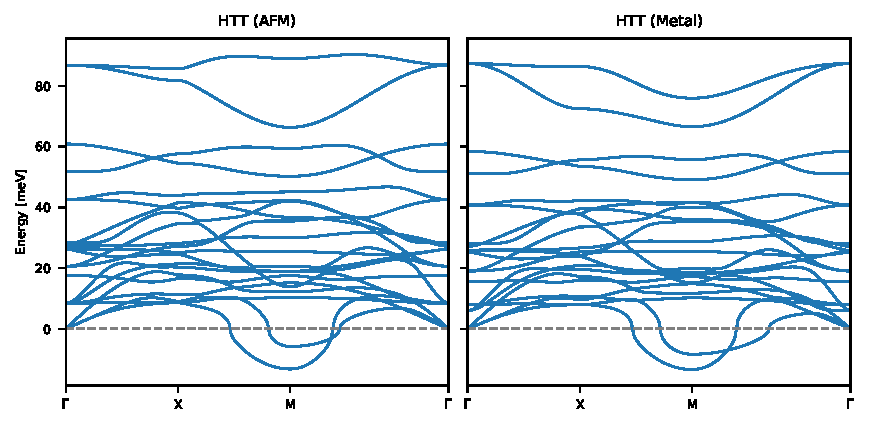
\includegraphics[width=\textwidth]{fig/simulation/htt_bands.pdf}
	\caption[HTT Bands]{Phonon band structure of LCO in the HTT phase using the PBESol functional and an 800 eV plane-wave cut-off. The high-symmetry lines are with respect to the primitive tetragonal BZ (See Figure \ref{fig:band_paths})}
	\label{fig:htt_bands}
\end{figure}

While there, in principle, are a huge number of functionals one could try, phonon calculations are quite expensive and the PBESol results are reasonable in the context of lattice dynamics. We thus stick to the PBESol functional in simulations moving forward. To check the stability of structural phases in LCO, we perform phonon calculation in the LTO and LTT phases, shown in Figure \ref{fig:lto_bands} and \ref{fig:ltt_bands}. Qualitatively, we see similar features to HTT (apart from the obvious increase of bands). The most significant result is that the LTO and LTT phases clearly stabilizes at the $M$-point, suggesting that our simulations reproduce the observed structural phase transitions. The stability of LTT is particularly interesting in this case, since this phase is believed to suppress superconductivity. In particular when combined with the fact that LTO and LTT are very close in energy when looking at the metallic simulations.

\begin{figure}
	\centering
	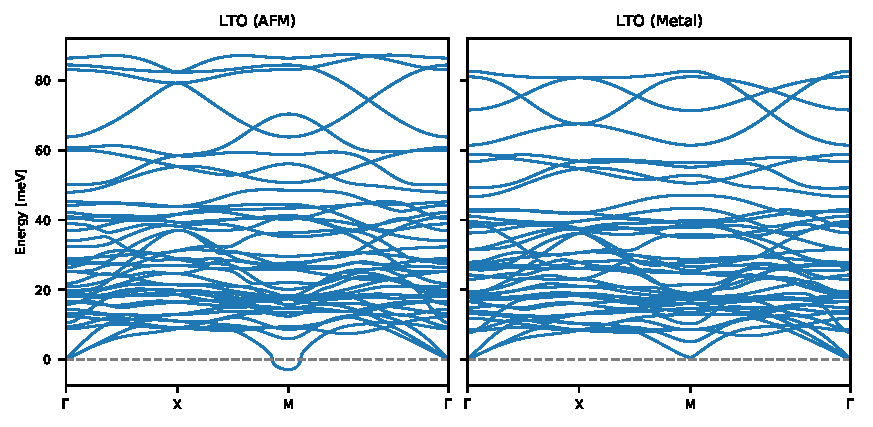
\includegraphics[width=\textwidth]{fig/simulation/lto_bands.pdf}
	\caption[LTO Bands]{Phonon band structure of LCO in the LTO phase using the PBESol functional and an 800 eV plane-wave cut-off. The high-symmetry lines are with respect to the primitive tetragonal BZ (See Figure \ref{fig:band_paths})}
	\label{fig:lto_bands}
\end{figure}

\begin{figure}
	\centering
	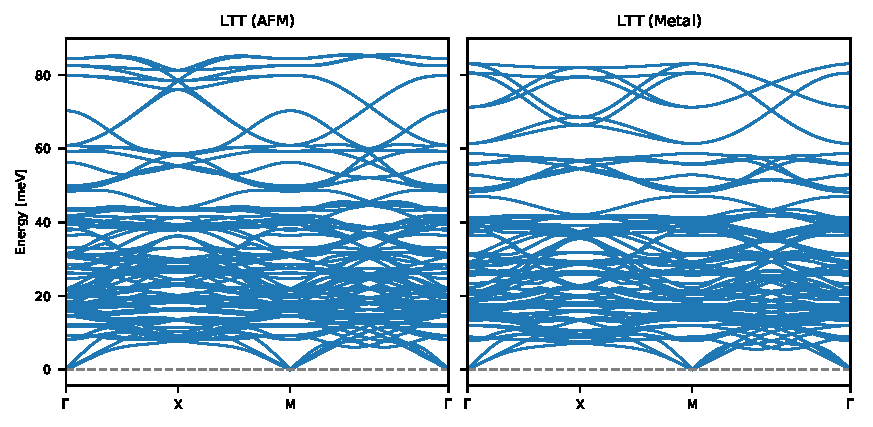
\includegraphics[width=\textwidth]{fig/simulation/ltt_bands.pdf}
	\caption[LTT Bands]{Phonon band structure of LCO in the LTT phase using the PBESol functional and an 800 eV plane-wave cut-off. The high-symmetry lines are with respect to the primitive tetragonal BZ (See Figure \ref{fig:band_paths})}
	\label{fig:ltt_bands}
\end{figure}

\subsection{Density of states}\label{sec:sim_dos}
As discussed in section [REF], the the calculation of phonon bands makes it trivial to compute the (partial) phonon DOS by evaluating the bands on a grid and integrating onto the energy axis. By evaluating the partial DOS and weighing each partial by scattering cross section ($\sigma^\text{total}$) and ionic mass, we obtain the generalized phonon DOS as seen by a time-of-flight neutron spectrometer in the incoherent approximation. 

\begin{figure}
	\centering
	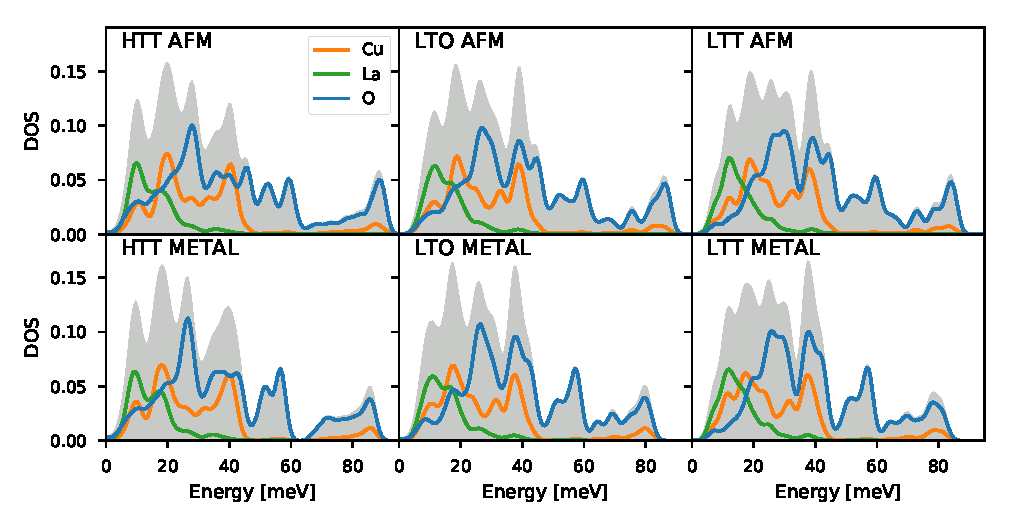
\includegraphics[width=\textwidth]{fig/simulation/phonopy_pdos.pdf}
	\caption[Neutron DOS (frozen-phonons)]{Neutron-weighted phonon density of states in the various structural and electronic phases of LCO. Both the partial and total density of states is shown in the plot.}
	\label{fig:dos_all}
\end{figure}

Figure \ref{fig:dos_all} shows the neutron weighted partial and total density of states due to the 6 different phonon calculations we performed. The density of states was evaluated on a $48 \times 48 \times 48$ grid, integrated using the tetrahedron method and an applied Gaussian smearing of $\sigma=\SI{1}{\milli\eV}$ (\SI{2.35}{\milli\eV} FWHM). To get comparable values of $g(\omega)$, the plots are normalized to the BZ volume ($4V^\text{BZ}_\text{HTT} = 2 V^\text{BZ}_\text{LTO} = V^\text{BZ}_\text{LTT}$).

Qualitatively, the main difference between the structural phases is a modification of the peak at $\approx \SI{30}{\milli\eV}$ as you go to progressively lower symmetries. A quick inspection of the eigenvectors of the HTT calculation reveals 4 modes in this energy-range (inspection performed at $\Gamma$)\todo{visual}:

\begin{enumerate}
	\item \SI{26.3}{\milli\eV}: An in-plane oxygen mode where the oxygens move along $c$ and the two diagonals of the octahedra is out of phase.
	\item \SI{27.2}{\milli\eV}: An apical oxygen mode where apical of the same `plane' move together with the direction alternating between each plane
	\item \SI{27.9}{\milli\eV}: A mode where every oxygen-atom moves in-phase along $c$, keeping the rest of the lattice still.
	\item \SI{28.6}{\milli\eV}: A lanthanum mode where the atoms move out of phase along $c$.
\end{enumerate}

The metallic simulations mainly have the effect of generally pushing phonon energies down and a `smoothing' of high-energy modes. Extrapolating from the HTT phase, this is directly linked to the softening of the Cu-O bond-stretching mode at the zone boundary, as will be discussed in chapter \ref{ch:anomaly}. In addition, the two peaks at \SI{50}{\milli\eV} and \SI{60}{\milli\eV} have weight shifted towards the latter. The mode at \SI{50}{\milli\eV} is a bond-stretching mode of the apical oxygen, while the mode at \SI{60}{\milli\eV} involves vibration of all oxygen-atoms along the $c$ axis, with in-plane and apical oxygen atoms being relatively out of phase.

\section{Validation of simulations}\label{sec:sim_validation}
Since LSCO is such an extensively studied system, there is data available in the literature to compare our band structures. By inspection of the band structure plots in the previous section, it seems like a difficult task to actually separate the bands in a neutron scattering experiment. Luckily, there are a few modes that can be distinguished. Figure \ref{fig:htt_phonons_lit} compares our HTT band phonons band structures along $\Gamma$-$X$ with experimental data from a range of LSCO samples. The highlighted modes is the Cu-O half-breathing mode ($\approx \SI{80}{\milli\eV}$) and the apical oxygen stretching mode ($\approx \SI{60}{\milli\eV}$). We will discuss this mode in detail in Chapter \ref{ch:anomaly}

\begin{figure}
	\centering
	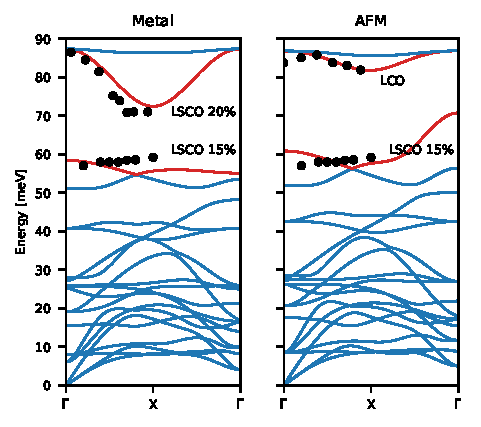
\includegraphics[width=0.7\textwidth]{fig/simulation/htt_phonons_lit.pdf}
	\caption[phonon bands: comparison with literature]{Comparison of phonon band structures in the HTT structural phase along the $\Gamma$-X path with data from literature. Data for LSCO 15\% taken from ref. \cite{McQueeney1999}, data for LSCO 20\% and 0\% taken from ref. \cite{Park2014}. Modes associated with data are highlighted in red.}
	\label{fig:htt_phonons_lit}
\end{figure}

Further validation of our simulations are performed in the experimental Chapters \ref{ch:lowen} and \ref{ch:in4} where we look at low-energy phonon modes and density-of-states measurements, respectively. In addition, some of the ideas developed here will be used in the investigation of simulations with O/Sr defects using ab-initio MD in the following chapter.

\section{Summary}
I summary, we performed ab-initio phonon calculations of La$_2$CuO$_4$ in 3 structural and two electronic phases, using the PBESol functional and an increased plane wave energy cut-off in order to correctly stabilize low-energy phonons. We discover imaginary modes at the $M$ point of the HTT, consistent with the observation of the HTT-LTO structural phase transition due to octahedral tilts. The relationship between the LTO and LTT phases are less consistent and we get different results for the metallic and AFM solutions. For the AFM case, LTT is the stable phase (and LTO is `less stable' compared to HTT), never seen in experiments on the undoped compound. In fact, the orthorhombic strain and octahedral tilt are both largest at zero doping \cite{Radaelli1994a}. For the metallic case, LTO and LTT are nearly degenerate (indistinguishable energies within our numerical precision), while experiments tells us that HTT is the stable phase at overdoing, at least for La$_{2-x}$Sr$_x$CuO$_4$.

Despite our results being inconsistent with regards to total energies and observed structural phases, we proceed our investigations based on the computational parameters decided on throughout this chapter. There are two reasons for this. First, we have a remarkable agreement with phonons at both high (chapter \ref{ch:anomaly} and Figure \ref{fig:htt_phonons_lit}) and low (Chapter \ref{ch:lowen}) energies. Second, we \emph{know} that a one-electron theory such as DFT is unable to explain the correlated nature of the cuprates at optimal doping, so we settle on the best description possible in the edge cases and try to extrapolate from that. The electronic structure of the cuprates at intermediate doping is essentially an unsolved problem outside the scope of this thesis.